\documentclass[aspectratio=169, 10pt]{beamer}

% --- Configurações Básicas e Idioma ---
\usepackage[utf8]{inputenc}
\usepackage[T1]{fontenc}
\usepackage[brazilian]{babel}
\usepackage{lmodern}

% --- Pacotes Matemáticos e Tipográficos ---
\usepackage{amsmath,amssymb,amsfonts}
\usepackage{booktabs,array,multirow,colortbl}
\usepackage{graphicx}
\usepackage{tikz}
\usetikzlibrary{shapes.geometric, arrows.meta, positioning}
\usepackage{pifont} % Para ícones de checkmark e xmark
\usepackage{microtype}

% --- Tema Madrid e Paleta em Tons de Azul Nobre ---
\usetheme{Madrid}
\usecolortheme{whale}

% Definição de Cores Personalizadas em Tons de Azul
\definecolor{DarkBlue}{RGB}{18, 48, 86}      % Azul Marinho Profundo
\definecolor{MedBlue}{RGB}{32, 90, 140}      % Azul Médio Principal
\definecolor{SoftBlue}{RGB}{232, 242, 250}   % Azul Suave para fundos
\definecolor{AccentBlue}{RGB}{0, 120, 185}   % Azul Ciano Destaque
\definecolor{NavyText}{RGB}{12, 30, 54}      % Azul Escuro para Texto
\definecolor{StatusGreen}{RGB}{34, 139, 34}  % Verde para OK
\definecolor{StatusAmber}{RGB}{210, 105, 30} % Âmbar para Alerta/Tratado

% Configuração das Cores do Beamer
\setbeamercolor{structure}{fg=MedBlue}
\setbeamercolor{palette primary}{bg=DarkBlue,fg=white}
\setbeamercolor{palette secondary}{bg=MedBlue,fg=white}
\setbeamercolor{palette tertiary}{bg=DarkBlue!85!black,fg=white}
\setbeamercolor{titlelike}{parent=palette primary,fg=white}
\setbeamercolor{frametitle}{bg=DarkBlue,fg=white}
\setbeamercolor{author in head/foot}{bg=DarkBlue!90!black,fg=white}
\setbeamercolor{title in head/foot}{bg=MedBlue,fg=white}
\setbeamercolor{date in head/foot}{bg=DarkBlue,fg=white}

% Blocos Customizados em Tons de Azul
\setbeamercolor{block title}{bg=MedBlue,fg=white}
\setbeamercolor{block body}{bg=SoftBlue!50,fg=NavyText}
\setbeamercolor{block title example}{bg=DarkBlue,fg=white}
\setbeamercolor{block body example}{bg=SoftBlue!30,fg=NavyText}
\setbeamercolor{block title alerted}{bg=red!75!DarkBlue,fg=white}
\setbeamercolor{block body alerted}{bg=red!8,fg=NavyText}

% Configuração de Itens e Símbolos
\setbeamertemplate{items}[circle]
\setbeamertemplate{navigation symbols}{} % Remove botões de navegação poluídos

% Comandos auxiliares de status
\newcommand{\cmark}{\textcolor{StatusGreen}{\ding{51}}}
\newcommand{\tmark}{\textcolor{StatusAmber}{\ding{115}}}

% --- Metadados da Apresentação ---
\title[PCC170 --- Entrega 2: Resultados Preliminares]{Efeitos do Uso de Inteligência Artificial, Ansiedade e Estudo Tradicional no Rendimento Acadêmico (\texorpdfstring{$\Delta \text{GPA}$}{Delta GPA})}
\subtitle{Resultados Preliminares --- Projeto Fatorial $2^3 r$ com Análise Individual de Casos}
\author[Wagner T. P.]{Wagner Tironi Pinto}
\institute[UFOP - DECOM]{
    Programa de Pós-Graduação em Ciência da Computação (PPGCC) \\
    Universidade Federal de Ouro Preto (UFOP) \\
    \medskip
    \textit{Disciplina: PCC170 --- Projeto e Análise de Experimentos Computacionais} \\
    \textit{Prof. Carlos Henrique Gomes Ferreira}
}
\date{\today}

% ==============================================================================
% DOCUMENTO
% ==============================================================================
\begin{document}

% ------------------------------------------------------------------------------
% Slide 1: Capa
% ------------------------------------------------------------------------------
\begin{frame}[plain]
    \titlepage
\end{frame}

% ------------------------------------------------------------------------------
% Slide 2: Contextualização e Motivação
% ------------------------------------------------------------------------------
\begin{frame}{1. Contextualização e Motivação}
    \begin{columns}[T]
        \begin{column}{0.48\textwidth}
            \begin{block}{O Paradoxo da IA na Educação}
                \begin{itemize}\setlength{\itemsep}{5pt}
                    \item A adoção massiva de ferramentas de IA generativa no ensino superior.
                    \item \textbf{Dilema central:} O uso da IA como tutor (estudo ativo) versus o uso como atalho (cópia passiva).
                    \item Risco de os alunos pensarem menos por conta própria, prejudicando o aprendizado a longo prazo.
                \end{itemize}
            \end{block}

            \begin{block}{Interações Comportamentais}
                \begin{itemize}
                    \item A tecnologia não atua isolada: dedicação ao estudo tradicional e controle de ansiedade modulam o impacto final no GPA.
                \end{itemize}
            \end{block}
        \end{column}

        \begin{column}{0.48\textwidth}
            \begin{block}{Abordagem Metodológica (DoE)}
                \begin{itemize}\setlength{\itemsep}{5pt}
                    \item Estruturação via \textbf{Projeto de Experimentos Computacionais}:
                    \begin{itemize}
                        \item Avaliar o impacto de cada fator isoladamente e combinados.
                        \item Análise controlada com correção de heterocedasticidade.
                    \end{itemize}
                    \item \textbf{Meta:} Oferecer evidências empíricas para guiar políticas pedagógicas na universidade.
                \end{itemize}
            \end{block}
            \begin{exampleblock}{População Alvo}
                Estudantes de graduação em \textbf{STEM} no 3º ano (\textit{Junior}), período crítico de consolidação disciplinar.
            \end{exampleblock}
        \end{column}
    \end{columns}
\end{frame}

% ------------------------------------------------------------------------------
% Slide 3: Pergunta de Pesquisa e Hipótese Geral
% ------------------------------------------------------------------------------
\begin{frame}{2. Pergunta de Pesquisa e Hipótese Geral}
    \begin{block}{Pergunta Orientadora da Pesquisa}
        \textit{De que maneira o modo de uso de IA, o nível de ansiedade em avaliações e as horas de estudo tradicional se combinam para influenciar o ganho de rendimento acadêmico ($\Delta \text{GPA}$) em estudantes STEM?}
    \end{block}

    \vspace{4pt}

    \begin{exampleblock}{Hipótese Geral Formulada \textit{A Priori}}
        \textbf{H:} \textit{O ganho acadêmico ($\Delta \text{GPA}$) é condicionado conjuntamente pelos três fatores. Espera-se que o uso ativo de IA e o maior estudo tradicional elevem o $\Delta \text{GPA}$, enquanto o uso passivo e a ansiedade elevada o reduzam, com uma piora acentuada quando o uso passivo se junta à alta ansiedade ($A \times B$).}
    \end{exampleblock}

    \vspace{4pt}

    \begin{alertblock}{Os Limites do Estudo}
        Como os dados são observacionais (sem a divisão aleatória dos alunos), os resultados indicam associações fortes entre os hábitos e as notas, mas não comprovam a causalidade direta.
    \end{alertblock}
\end{frame}

% ------------------------------------------------------------------------------
% Slide 4: Estrutura Experimental 2^3 r
% ------------------------------------------------------------------------------
\begin{frame}{3. Estrutura Experimental $2^3 r$ e a Variável de Resposta}
    \begin{columns}[T]
        \begin{column}{0.4\textwidth}
            \begin{block}{Definição da Unidade e Resposta}
                \begin{itemize}\setlength{\itemsep}{6pt}
                    \item \textbf{Unidade Experimental:} Aluno individual (\texttt{Student\_ID} único).
                    \item \textbf{Variável Resposta:}
                    $$\Delta \text{GPA} = \text{GPA}_{\text{pós-semest}} - \text{GPA}_{\text{pré-semest}}$$
                    \item \textbf{Vantagem Analítica:} Mede a evolução marginal de cada estudante, controlando a linha de base individual.
                    \item \textbf{Escala:} GPAs contidos em $[0.0, 4.0]$.
                \end{itemize}
            \end{block}
        \end{column}

        \begin{column}{0.55\textwidth}
            \begin{block}{Fatores e Codificação Matricial ($\pm 1$)}
                \centering \small  
                \begin{tabular}{lll}
                    \toprule
                    \textbf{Fator} & \textbf{Nível $-1$} & \textbf{Nível $+1$} \\
                    \midrule
                    \textbf{A: Uso de IA} & Ativo (tutoria) & Passivo (\textit{copy/direct}) \\
                    \textbf{B: Ansiedade} & Baixa ($\le Q_2$) & Alta ($> Q_2=4$) \\
                    \textbf{C: Estudo Trad.} & Baixo ($\le Q_2$) & Alto ($> Q_2=10,91\text{h}$) \\
                    \bottomrule
                \end{tabular}
            \end{block}

            \begin{exampleblock}{Projeto Fatorial Completo}
                \begin{itemize}
                    \item $k = 3$ fatores $\implies 2^3 = 8$ combinações experimentais.
                    \item Dicotomização pela mediana amostral de STEM Junior.
                \end{itemize}
            \end{exampleblock}
        \end{column}
    \end{columns}
\end{frame}

% ------------------------------------------------------------------------------
% Slide 5: Auditoria de Integridade e Viabilidade Amostral (Quadro Nativo LaTeX)
% ------------------------------------------------------------------------------
\begin{frame}{4. Auditoria de Integridade e Viabilidade Amostral}
    \begin{columns}[T]
        \begin{column}{0.50\textwidth}
            \begin{block}{Quadro de Auditoria de Sanidade da Base}
                \centering \small
                \begin{tabular}{lcc}
                    \toprule
                    \textbf{Checagem de Qualidade} & \textbf{Ocorrências} & \textbf{Status} \\
                    \midrule
                    Identificadores (\texttt{ID}) duplicados & $0$ & \cmark\ \textbf{OK} \\
                    Campos críticos ausentes/\textit{NaN} & $0$ & \cmark\ \textbf{OK} \\
                    GPA fora do limite $[0.0, 4.0]$ & $0$ & \cmark\ \textbf{OK} \\
                    Valores negativos de estudo tradicional & $0$ & \cmark\ \textbf{OK} \\
                    Escala de ansiedade válida $[1, 10]$ & $0$ falhas & \cmark\ \textbf{OK} \\
                    \bottomrule
                \end{tabular}
            \end{block}

            \begin{block}{Composição do Fluxo Amostral}
                \centering
                \begin{tikzpicture}[node distance=0.6cm, auto, scale=0.8, every node/.style={transform shape}]
                    \node[draw=DarkBlue, fill=SoftBlue!40, rounded corners, inner sep=4pt, align=center] (b1) {\textbf{Base Total}\\\small $N = 50.000$};
                    \node[draw=DarkBlue, fill=SoftBlue!70, rounded corners, inner sep=4pt, right=of b1, align=center] (b2) {\textbf{STEM + Junior}\\\small $n = 3.279$};
                    \node[draw=DarkBlue, fill=MedBlue, text=white, rounded corners, inner sep=4pt, right=of b2, align=center] (b3) {\textbf{Células $2^3$}\\\small $n = 3.279$};
                    \draw[-{Stealth[length=2mm]}, thick, DarkBlue] (b1) -- (b2);
                    \draw[-{Stealth[length=2mm]}, thick, DarkBlue] (b2) -- (b3);
                \end{tikzpicture}
            \end{block}
        \end{column}

        \begin{column}{0.48\textwidth}
            \begin{block}{Garantia de Réplicas ($r \ge 10$)}
                \begin{itemize}\setlength{\itemsep}{5pt}
                    \item Exigência regulamentar da disciplina: $r \ge 10$ réplicas por vértice.
                    \item \textbf{Célula com menor tamanho:} $n_{\min} = 181$ alunos (célula \texttt{ab}).
                    \item \textbf{Célula com maior tamanho:} $n_{\max} = 667$ alunos (célula \texttt{c}).
                    \item Margem estatística: mais de \textbf{18 vezes superior} ao limiar obrigatório.
                \end{itemize}
            \end{block}

            \begin{exampleblock}{Conclusão de Viabilidade}
                Base íntegra, sem descarte artificial de dados e com elevado poder de precisão estimativa.
            \end{exampleblock}
        \end{column}
    \end{columns}
\end{frame}

% ------------------------------------------------------------------------------
% Slide 6: Primeiros Resultados do 2^3: Cubo Fatorial e Células
% ------------------------------------------------------------------------------
\begin{frame}{5. Primeiros Resultados: Espaço Fatorial}
    
    \begin{block}{Médias e Desvios}
        \centering
        % O comando resizebox correto envolve toda a tabela
        \resizebox{\textwidth}{!}{%
        \begin{tabular}{llccr}
            \toprule
            \textbf{Ensaio} & \textbf{Código} & \textbf{Perfil} & $n$ & \textbf{Média $\pm$ DP} \\
            \midrule
            \texttt{(1)} & $(-1,-1,-1)$ & Ativo, Ans. Baixa, Est. Baixo & 442 & $-0.021 \pm 0.20$ \\
            \texttt{a}   & $(+1,-1,-1)$ & Pass., Ans. Baixa, Est. Baixo & 225 & $-0.089 \pm 0.21$ \\
            \texttt{b}   & $(-1,+1,-1)$ & Ativo, Ans. Alta, Est. Baixo  & 382 & $-0.029 \pm 0.20$ \\
            \texttt{ab}  & $(+1,+1,-1)$ & Pass., Ans. Alta, Est. Baixo  & 181 & $\mathbf{-0.134} \pm 0.22$ \\
            \texttt{c}   & $(-1,-1,+1)$ & Ativo, Ans. Baixa, Est. Alto  & 667 & $\mathbf{+0.104} \pm 0.21$ \\
            \texttt{ac}  & $(+1,-1,+1)$ & Pass., Ans. Baixa, Est. Alto  & 371 & $+0.024 \pm 0.19$ \\
            \texttt{bc}  & $(-1,+1,+1)$ & Ativo, Ans. Alta, Est. Alto   & 614 & $+0.088 \pm 0.20$ \\
            \texttt{abc} & $(+1,+1,+1)$ & Pass., Ans. Alta, Est. Alto   & 397 & $+0.028 \pm 0.20$ \\
            \bottomrule
        \end{tabular}%
        } % Fim do resizebox
    \end{block}
    
    \vspace{0.3cm} % Respiro entre o bloco e os itens
    
    \begin{itemize}
        \item \textbf{Pior cenário:} \texttt{ab} ($\mu = -0.134$): passivo + ansioso + estudo baixo.
        \item \textbf{Melhor cenário:} \texttt{c} ($\mu = +0.104$): ativo + não ansioso + estudo alto.
    \end{itemize}
    
\end{frame}

% ------------------------------------------------------------------------------
% Slide 7: ECDF Individual — Fator A
% ------------------------------------------------------------------------------
\begin{frame}{6. Distribuição Acumulada (ECDF): Modo de Uso de IA (Fator A)}
    \begin{columns}[c]
        \begin{column}{0.50\textwidth}
            \centering
            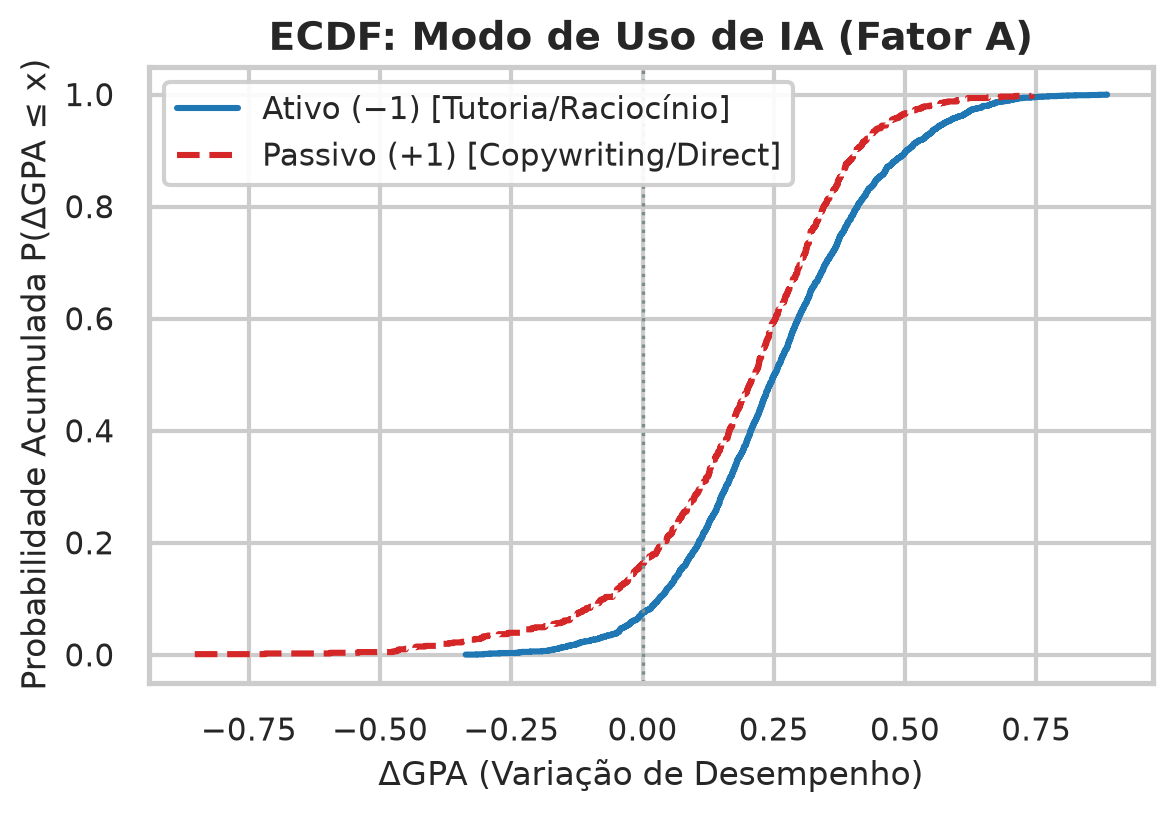
\includegraphics[width=\linewidth, height=0.68\textheight, keepaspectratio]{figuras/02_ecdf_fator_A.png}
            \vspace{-4pt}
            {\tiny \textbf{Figura 2A:} Função de distribuição cumulativa empírica para o Fator A.}
        \end{column}

        \begin{column}{0.48\textwidth}
            \begin{block}{Explicação Objetiva do Caso A}
                \begin{itemize}\setlength{\itemsep}{5pt}\small
                    \item \textbf{Curva Vermelha tracejada (Passivo):} Percebe-se o deslocamento para a esquerda em relação à azul (Ativo).
                    \item \textbf{Maior Fração Negativa:} Os estudantes com o uso passivo apresentam probabilidade estocasticamente superior de queda de GPA ($\Delta \text{GPA} < 0$).
                    \item \textbf{Regularidade:} Curvas contínuas sem assimetrias abruptas ou outliers espúrios.
                \end{itemize}
            \end{block}
            \begin{exampleblock}{Conclusão Exploratória}
                Os estudantes que usam a IA de forma passiva têm uma chance consideravelmente maior de verem suas notas caírem em comparação com os que usam de forma ativa.
            \end{exampleblock}
        \end{column}
    \end{columns}
\end{frame}

% ------------------------------------------------------------------------------
% Slide 8: ECDF Individual — Fator B
% ------------------------------------------------------------------------------
\begin{frame}{7. Distribuição Acumulada (ECDF): Ansiedade em Provas (Fator B)}
    \begin{columns}[c]
        \begin{column}{0.50\textwidth}
            \centering
            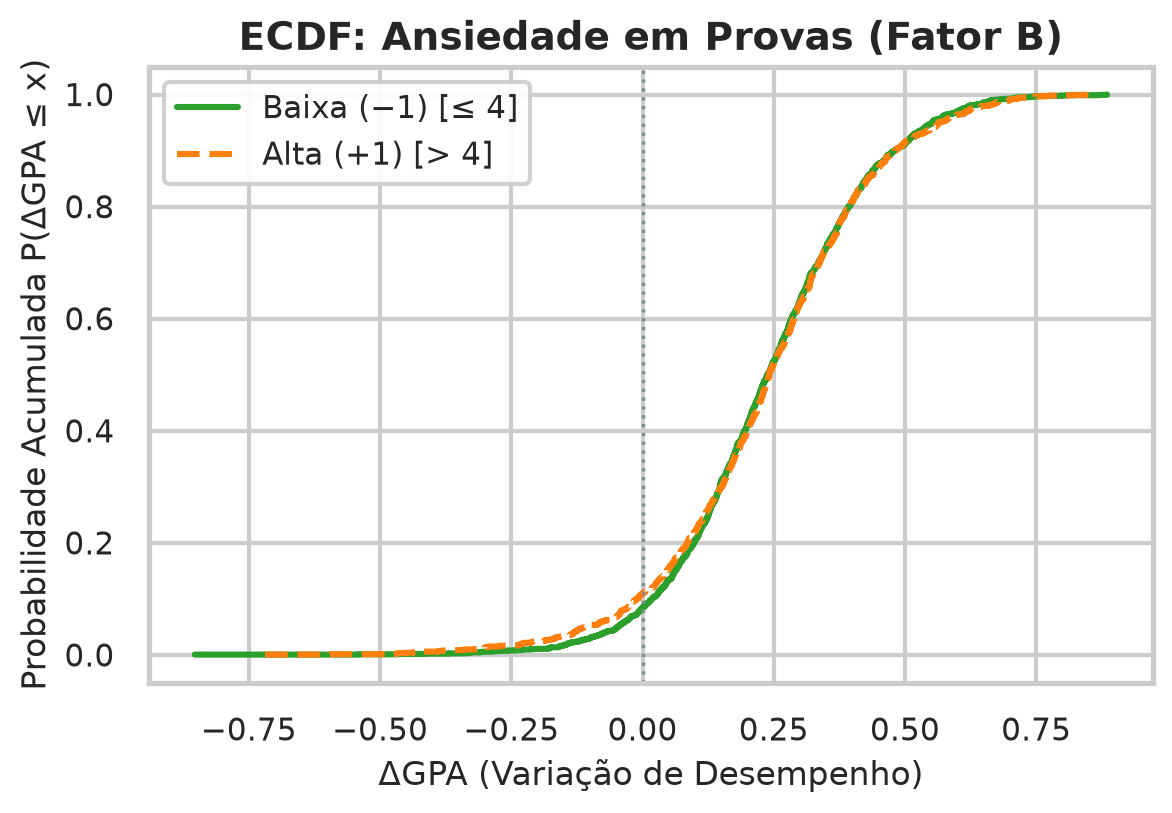
\includegraphics[width=\linewidth, height=0.68\textheight, keepaspectratio]{figuras/02_ecdf_fator_B.png}
            \vspace{-4pt}
            {\tiny \textbf{Figura 2B:} Função de distribuição cumulativa empírica para o Fator B.}
        \end{column}

        \begin{column}{0.48\textwidth}
            \begin{block}{Explicação Objetiva do Caso B}
                \begin{itemize}\setlength{\itemsep}{5pt}\small
                    \item \textbf{Curva Laranja tracejada (Alta Ansiedade):} Apresenta um leve deslocamento negativo em relação à curva verde, indicando uma sutil desvantagem.
                    \item \textbf{Efeito Moderado:} A forte sobreposição das curvas demonstra que a ansiedade, por si só, afeta muito pouco a variação do desempenho.
                    \item \textbf{Comportamento nos Extremos:} O comportamento dos alunos é muito semelhante em toda a trajetória.
                \end{itemize}
            \end{block}
            \begin{exampleblock}{Conclusão Exploratória}
                Ansiedade alta é desfavorável, mas sua ação ganha relevância quando combinada aos outros hábitos.
            \end{exampleblock}
        \end{column}
    \end{columns}
\end{frame}

% ------------------------------------------------------------------------------
% Slide 9: ECDF Individual — Fator C
% ------------------------------------------------------------------------------
\begin{frame}{8. Distribuição Acumulada (ECDF): Estudo Tradicional (Fator C)}
    \begin{columns}[c]
        \begin{column}{0.50\textwidth}
            \centering
            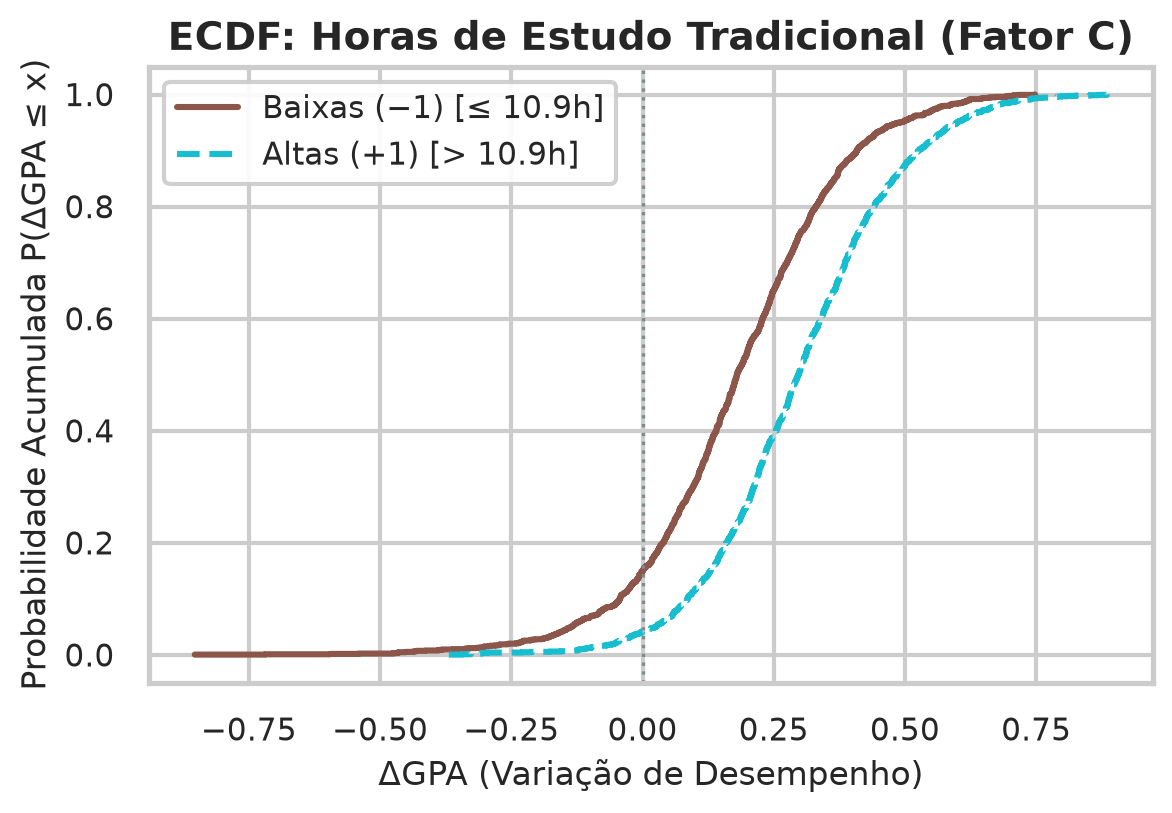
\includegraphics[width=\linewidth, height=0.68\textheight, keepaspectratio]{figuras/02_ecdf_fator_C.png}
            \vspace{-4pt}
            {\tiny \textbf{Figura 2C:} Função de distribuição cumulativa empírica para o Fator C.}
        \end{column}

        \begin{column}{0.48\textwidth}
            \begin{block}{Explicação Objetiva do Caso C}
                \begin{itemize}\setlength{\itemsep}{5pt}\small
                    \item \textbf{Dominância Estocástica Nítida:} A curva ciano posiciona-se inteiramente à direita da marrom, indicando a superioridade do alto volume de estudo.
                    \item \textbf{Proteção Universal:} Em qualquer cenário de corte, a proporção de alunos com melhora nas notas é maior no nível +1.
                    \item \textbf{Força Preditiva:} Este é o fator que apresenta a maior separação visual entre as curvas, indicando seu forte peso individual.
                \end{itemize}
            \end{block}
            \begin{exampleblock}{Conclusão Exploratória}
                O estudo tradicional atua como a principal alavanca isolada para o ganho de rendimento acadêmico.
            \end{exampleblock}
        \end{column}
    \end{columns}
\end{frame}

% ------------------------------------------------------------------------------
% Slide 10: Efeito Principal do Fator C
% ------------------------------------------------------------------------------
\begin{frame}{9. Efeito Principal do Fator C: Horas de Estudo Tradicional}
    \begin{columns}[c]
        \begin{column}{0.50\textwidth}
            \centering
            \includegraphics[width=\linewidth, height=0.68\textheight, keepaspectratio]{figuras/06_efeito_principal_C.png}
            \vspace{-4pt}
            {\tiny \textbf{Figura 3C:} Médias balanceadas de $\Delta \text{GPA}$ para o Fator C (Estudo Tradicional).}
        \end{column}

        \begin{column}{0.48\textwidth}
            \begin{block}{Quantificação do Contraste}
                \begin{itemize}\setlength{\itemsep}{5pt}\small
                    \item \textbf{Média Estudo Baixo (-1)}: $+0.160$ (até 10,9 h/sem)
                    \item \textbf{Média Estudo Alto (+1)}: $+0.281$ (mais de 10,9 h/sem)
                    \item \textbf{Efeito principal ($\Delta$):} $\mathbf{+0.121}$ pontos no GPA
                    \item \textbf{Validação Estatística:} Resultado altamente significativo ($p < 0.0001$), com Intervalo de Confiança (95) entre $[+0.106 \text{ e } +0.136]$.
                \end{itemize}
            \end{block}
            \begin{exampleblock}{Impacto Prático}
                É o \textbf{fator de maior peso no desempenho}: estudar acima da mediana (10,9h) garante um ganho líquido médio isolado de $+0.121$ pontos na nota, independentemente de outros hábitos.
            \end{exampleblock}
        \end{column}
    \end{columns}
\end{frame}

% ------------------------------------------------------------------------------
% Slide 11: Efeito Principal do Fator A
% ------------------------------------------------------------------------------
\begin{frame}{10. Efeito Principal do Fator A: Modo de Uso de IA}
    \begin{columns}[c]
        \begin{column}{0.50\textwidth}
            \centering
            \includegraphics[width=\linewidth, height=0.68\textheight, keepaspectratio]{figuras/06_efeito_principal_A.png}
            \vspace{-4pt}
            {\tiny \textbf{Figura 3A:} Médias balanceadas de $\Delta \text{GPA}$ para o Fator A (Modo de IA).}
        \end{column}

        \begin{column}{0.48\textwidth}
            \begin{block}{Quantificação do Contraste}
                \begin{itemize}\setlength{\itemsep}{5pt}\small
                    \item \textbf{Média Uso Ativo (-1):} $+0.259$ (Tutoria / Raciocínio) 
                    \item \textbf{Média Uso Passivo (+1):} $+0.182$ (Geração Direta / Copywriting)
                    \item \textbf{Efeito Principal ($\Delta$):} $\mathbf{-0.077}$ pontos no GPA 
                    \item \textbf{Validação Estatística:} Impacto estatisticamente significativo ($p < 0.0001$), com Intervalo de Confiança (95) entre $[-0.092 \text{ e } -0.062]$.
                \end{itemize}
            \end{block}
            \begin{alertblock}{Impacto Prático}
                Migrar do uso ativo para o passivo gera uma \textbf{penalização média de $-0.077$ pontos no GPA}, confirmando que a delegação passiva de tarefas reduz a retenção e o aprendizado. 
            \end{alertblock}
        \end{column}
    \end{columns}
\end{frame}

% ------------------------------------------------------------------------------
% Slide 12: Efeito Principal do Fator B
% ------------------------------------------------------------------------------
\begin{frame}{11. Efeito Principal do Fator B: Ansiedade em Provas}
    \begin{columns}[c]
        \begin{column}{0.50\textwidth}
            \centering
            \includegraphics[width=\linewidth, height=0.68\textheight, keepaspectratio]{figuras/06_efeito_principal_B.png}
            \vspace{-4pt}
            {\tiny \textbf{Figura 3B:} Médias balanceadas de $\Delta \text{GPA}$ para o Fator B (Ansiedade).}
        \end{column}

        \begin{column}{0.48\textwidth}
            \begin{block}{Quantificação do Contraste}
                \begin{itemize}\setlength{\itemsep}{5pt}\small
                    \item \textbf{Média Ansiedade Baixa (-1):} $+0.229$ (nota $\le 4$)
                    \item \textbf{Média Ansiedade Alta (+1):} $+0.212$ (nota $> 4$)
                    \item \textbf{Efeito Principal ($\Delta$):} $\mathbf{-0.0175}$ pontos no GPA
                    \item \textbf{Validação Estatística:} Impacto estatisticamente significativo ($p = 0.0268$), com Intervalo de Confiança (95) entre $[-0.033 \text{ e } -0.002]$.
                    %\item \textbf{Estatística de Teste:} $|t|_{\text{HC3}} = 2.22$ ($p = 0.0268$)
                \end{itemize}
            \end{block}
            \begin{exampleblock}{Impacto Prático}
                A alta ansiedade gera um impacto isolado reduzido ($-0.018$ pontos no GPA). Embora seja relevante ($p < 0.05$), indica que a ansiedade por si só não é o fator determinante no rendimento.
            \end{exampleblock}
        \end{column}
    \end{columns}
\end{frame}

% ------------------------------------------------------------------------------
% Slide 13: Interação A x B (Uso de IA x Ansiedade)
% ------------------------------------------------------------------------------
\begin{frame}{12. Interação Fatorial $A \times B$: Modo de Uso de IA $\times$ Ansiedade}
    \begin{columns}[c]
        \begin{column}{0.50\textwidth}
            \centering
            \includegraphics[width=\linewidth, height=0.68\textheight, keepaspectratio]{figuras/06_interacao_AB.png}
            \vspace{-4pt}
            {\tiny \textbf{Figura 4A:} Médias balanceadas para a interação $A \times B$.}
        \end{column}

        \begin{column}{0.48\textwidth}
            \begin{alertblock}{Quebra de Paralelismo (Sinergia Negativa)}
                \begin{itemize}\setlength{\itemsep}{5pt}\small
                    \item \textbf{Efeito de Interação ($A \times B$):} $\mathbf{-0.0226}$ ($p = 0.0041$)
                    \item \textbf{IC (95\% Bootstrap):} $[-0.038 \text{ e } -0.007]$ o que confirma efeito significativo.
                    \item Efeito Condicional da Mudança de Uso:
                    \begin{itemize}\footnotesize
                        \item Ansiedade Baixa: a transição de uso ativo para passivo reduz o GPA em apenas $-0.055$.
                        \item Ansiedade Alta: a mesma transição amplia a queda para $-0.100$.
                    \end{itemize}
                \end{itemize}
            \end{alertblock}
            \begin{exampleblock}{Impacto Prático}
                O uso passivo de IA potencializa os efeitos da ansiedade: a perda de rendimento acadêmico quase duplica (de $-0.055$ para $-0.100$) nos estudantes com alto estresse avaliativo. 
            \end{exampleblock}
        \end{column}
    \end{columns}
\end{frame}

% ------------------------------------------------------------------------------
% Slide 14: Interação A x C (Uso de IA x Estudo Tradicional)
% ------------------------------------------------------------------------------
\begin{frame}{13. Interação Fatorial $A \times C$: Modo de Uso de IA $\times$ Estudo Tradicional}
    \begin{columns}[c]
        \begin{column}{0.50\textwidth}
            \centering
            \includegraphics[width=\linewidth, height=0.68\textheight, keepaspectratio]{figuras/06_interacao_AC.png}
            \vspace{-4pt}
            {\tiny \textbf{Figura 4B:} Médias balanceadas para a interação $A \times C$.}
        \end{column}

        \begin{column}{0.48\textwidth}
            \begin{block}{Paralelismo Estrito (Efeitos Aditivos)}
                \begin{itemize}\setlength{\itemsep}{5pt}\small
                    \item \textbf{Efeito de Interação ($A \times C$):} $\mathbf{-0.0005}$ ($p = 0.9507$, não significativo)
                    \item \textbf{IC (95\% Bootstrap):} $[-0.016 \text{ e } +0.015]$ (perfeitamente centrado no zero).  
                    \item \textbf{Efeitos Estritamente Aditivos:}
                    \begin{itemize}\footnotesize
                        \item As retas são rigorosamente paralelas.
                        \item O ganho por estudar mais (nível $+1$) mantém-se fixo em $\mathbf{+0.121}$ pontos no GPA, tanto no uso ativo quanto no uso passivo de IA.  
                    \end{itemize}
                \end{itemize}
            \end{block}
            \begin{exampleblock}{Impacto Prático}
                O benefício do estudo tradicional atua de forma independente do modo de uso da IA: mais horas ao estudo garante o mesmo ganho de rendimento, independentemente da utilização da IA.
            \end{exampleblock}
        \end{column}
    \end{columns}
\end{frame}

% ------------------------------------------------------------------------------
% Slide 15: Interação B x C (Ansiedade x Estudo Tradicional)
% ------------------------------------------------------------------------------
\begin{frame}{14. Interação Fatorial $B \times C$: Ansiedade $\times$ Estudo Tradicional}
    \begin{columns}[c]
        \begin{column}{0.50\textwidth}
            \centering
            \includegraphics[width=\linewidth, height=0.68\textheight, keepaspectratio]{figuras/06_interacao_BC.png}
            \vspace{-4pt}
            {\tiny \textbf{Figura 4C:} Médias balanceadas para a interação $B \times C$.}
        \end{column}

        \begin{column}{0.48\textwidth}
            \begin{block}{Independência Estatística}
                \begin{itemize}\setlength{\itemsep}{5pt}\small
                    \item \textbf{Efeito de Interação ($B \times C$):} $\mathbf{+0.0107}$ ($p = 0.1766$, não significativo)
                    \item \textbf{IC 95\% Bootstrap:} $[-0.005 \text{ e } +0.026]$ (inclui o zero).
                    \item \textbf{Retas Paralelas:}
                    \begin{itemize}\footnotesize
                        \item As retas mantêm-se paralelas, mostrando que a resposta à ansiedade é a mesma em ambos os níveis de estudo.
                    \end{itemize}
                    \item Interação tripla $A \times B \times C = +0.0102$ ($p = 0.2178$) também sem significância.
                \end{itemize}
            \end{block}
            \begin{exampleblock}{Impacto Prático}
                Aumentar o tempo de estudo gera impacto positivo no rendimento, independentemente do estudante apresentar alta ou baixa ansiedade em provas.
            \end{exampleblock}
        \end{column}
    \end{columns}
\end{frame}

% ------------------------------------------------------------------------------
% Slide 16: Diagnósticos de Pressupostos (Quadro Nativo LaTeX)
% ------------------------------------------------------------------------------
\begin{frame}{15. Diagnósticos Estatísticos dos Pressupostos do Modelo}
    \begin{columns}[T]
        \begin{column}{0.54\textwidth}
            \begin{block}{Quadro de Auditoria dos Pressupostos}
                \centering \small
                \begin{tabular}{lcc}
                    \toprule
                    \textbf{Premissa / Teste} & \textbf{Estatística / $p$} & \textbf{Status / Conduta} \\
                    \midrule
                    Shapiro-Wilk (Resíduos) & $W = 0.999$, $p = 0.115$ & \cmark\ \textbf{Normalidade OK} \\
                    Levene (Dados Brutos) & $F = 4.73$, $p = 2.6 \times 10^{-5}$ & \tmark\ \textbf{Heterocedástico} \\
                    Levene (Réplicas Boot.) & $p = 0.044$ & \tmark\ \textbf{Boot. Estratificado} \\
                    Estabilidade de Sementes & Máx $\text{DP} = 0.0056$ & \cmark\ \textbf{Convergência OK} \\
                    GPA Prévio Balanceado & ANOVA $F=0.82$, $p > 0.05$ & \cmark\ \textbf{Sem viés inicial} \\
                    \bottomrule
                \end{tabular}
            \end{block}

            \begin{block}{Tratamento da Heterocedasticidade}
                \begin{itemize}\footnotesize
                    %\item \textbf{Erro-Padrão Sanduíche HC3 (MacKinnon-White):} Ajuste que penaliza resíduos de alta alavancagem em amostras desiguais.
                    \item Erros-Padrão Robustos (HC3): Correção do tipo "Sanduíche" para penalizar resíduos com alta alavancagem em amostras desiguais.
                    %\item \textbf{Bootstrap Estratificado:} $B=5.000$ iterações por célula.
                    \item Bootstrap Estratificado: Reamostragem ($B = 5.000$ iterações por célula) para assegurar que p-valores e intervalos de confiança não sejam subestimados.   
                \end{itemize}
            \end{block}
        \end{column}

        \begin{column}{0.44\textwidth}
            \begin{exampleblock}{Diagnóstico e Validação}
                \begin{itemize}\small
                    %\item Os resíduos atendem à normalidade ($p = 0.115$).
                    \item Normalidade dos Resíduos: Confirmada pelo teste de Shapiro-Wilk ($p = 0.115$), validando a distribuição do erro. 
                    %\item A heterocedasticidade observada ($p < 0.001$) reflete a natureza comportamental humana dos dados.
                    \item Variância Não-Constante: O teste de Levene indica heterocedasticidade ($p < 0.001$), comportamento esperado em dados comportamentais humanos. 
                    %\item O emprego de HC3 e Bootstrap garante que nenhum $p$-valor ou intervalo de confiança esteja subestimado.
                    \item Estabilidade Amostral: Balanceamento do GPA prévio confirmado via ANOVA ($p > 0.05$) e variação mínima entre sementes (Máx DP $= 0.0056$).
                \end{itemize}
            \end{exampleblock}
        \end{column}
    \end{columns}
\end{frame}

% ------------------------------------------------------------------------------
% Slide 17: Tabela de Inferência Consolidada (Slide Exclusivo em Largura Total)
% ------------------------------------------------------------------------------
\begin{frame}{16. Tabela de Inferência Consolidada dos Efeitos Fatoriais}
    \begin{block}{Resultados do Modelo Saturado $2^3$ (Erros HC3 e Bootstrap)}
        \centering
        \resizebox{\textwidth}{!}{%
        \renewcommand{\arraystretch}{1.15}
        \begin{tabular}{l c c c c c}
            \toprule
            \textbf{Termo Fatorial} & \textbf{Efeito ($\Delta$)} & \textbf{IC 95\% Bootstrap} & \textbf{Estatística $|t|_{\text{HC3}}$} & \textbf{$p$-valor (HC3)} & \textbf{Veredito} \\
            \midrule
            \rowcolor{SoftBlue!40}
            \textbf{C: Estudo Tradicional} & $\mathbf{+0.1211}$ & $[+0.106; +0.136]$ & $16.98$ & $< 0.0001$ & \cmark\ \textbf{Significativo (Dominante)} \\
            \rowcolor{SoftBlue!40}
            \textbf{A: Modo de Uso de IA} & $\mathbf{-0.0772}$ & $[-0.092; -0.062]$ & $10.49$ & $< 0.0001$ & \cmark\ \textbf{Significativo (Penalidade)} \\
            \rowcolor{SoftBlue!40}
            \textbf{AB: Interação IA $\times$ Ansiedade} & $\mathbf{-0.0226}$ & $[-0.038; -0.007]$ & $2.87$ & $0.0041$ & \cmark\ \textbf{Significativo (Sinergia)} \\
            \rowcolor{SoftBlue!40}
            \textbf{B: Ansiedade em Provas} & $\mathbf{-0.0175}$ & $[-0.033; -0.002]$ & $2.22$ & $0.0268$ & \cmark\ \textbf{Significativo (Efeito Reduzido)} \\
            \midrule
            \textbf{BC: Ansiedade $\times$ Estudo} & $+0.0107$ & $[-0.005; +0.026]$ & $1.35$ & $0.1766$ & Não Significativo \\
            \textbf{ABC: Interação Tripla} & $+0.0102$ & $[-0.006; +0.025]$ & $1.23$ & $0.2178$ & Não Significativo \\
            \textbf{AC: IA $\times$ Estudo} & $-0.0005$ & $[-0.016; +0.015]$ & $0.06$ & $0.9507$ & Não Significativo \\
            \bottomrule
        \end{tabular}%
        }
    \end{block}

    \vspace{4pt}

    \begin{exampleblock}{Síntese do Modelo}
        \small
        O modelo fatorial explica \textbf{$12,9\%$ da variância total} ($R^2 = 0.129$). Quatro efeitos são estatisticamente confirmados ($p_{\text{HC3}} < 0.05$ e ICs que excluem o zero), com destaque para o forte impacto do estudo tradicional e a penalidade do uso passivo de IA.
    \end{exampleblock}
\end{frame}

% ------------------------------------------------------------------------------
% Slide 17: Tabela de Inferência Consolidada (Slide Exclusivo em Largura Total)
% ------------------------------------------------------------------------------
\begin{frame}{16B. Distribuição dos Efeitos e Intervalos de Confiança Bootstrap}
    \centering
    % Inserção do gráfico ajustado à largura máxima útil do slide
    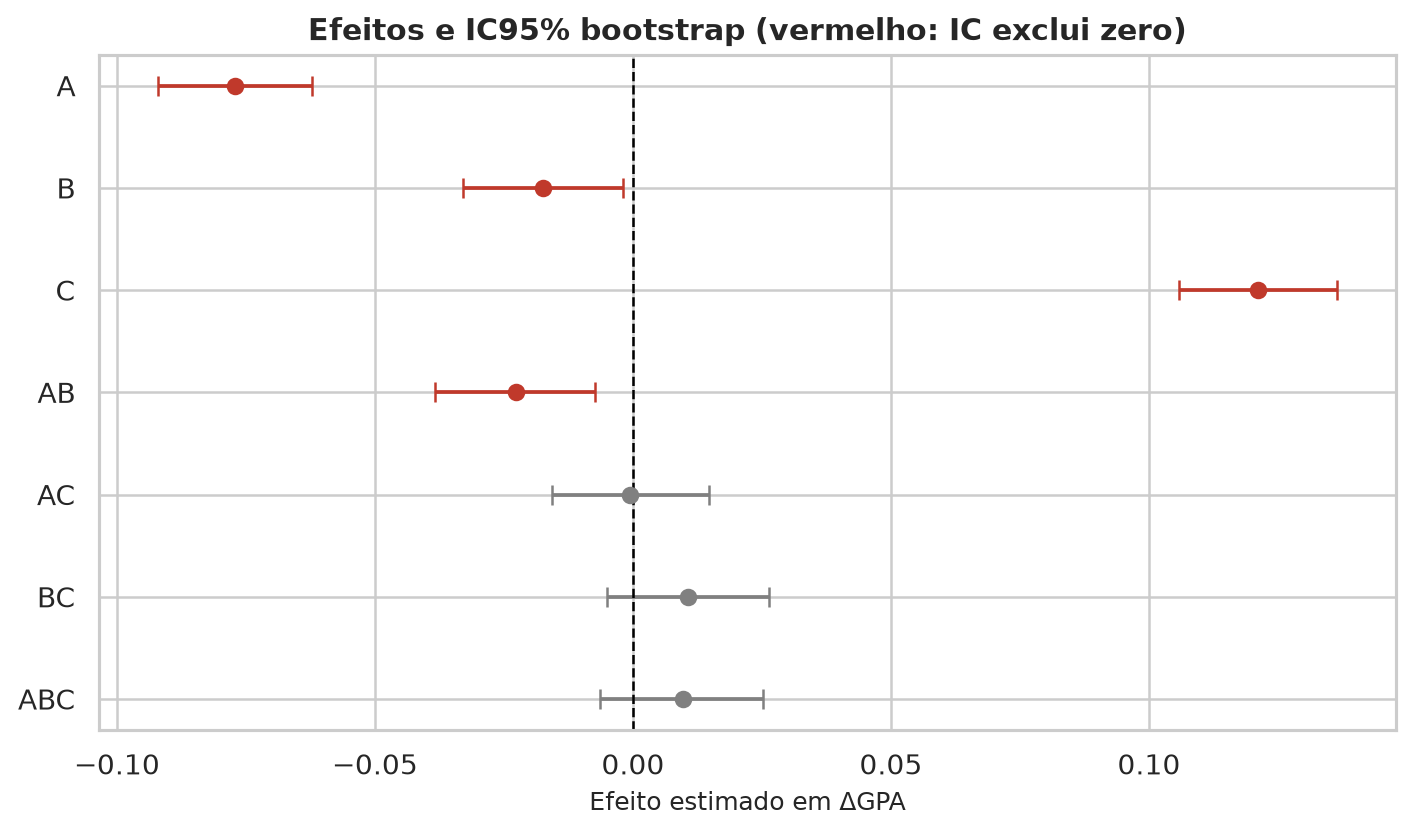
\includegraphics[width=0.92\textwidth, height=0.68\textheight, keepaspectratio]{figuras/07_forest_plot_relatorio.png}

    \vspace{4pt}

    \begin{exampleblock}{Síntese Visual da Inferência}
        \small
        \centering
        \textbf{Em vermelho:} Termos cujos ICs de 95\% excluem o zero ($p < 0.05$). \quad
        \textbf{Em cinza:} Termos nulos ($p > 0.05$).
    \end{exampleblock}
\end{frame}

% ------------------------------------------------------------------------------
% Slide 18: Diagrama de Pareto dos Efeitos Robustos HC3
% ------------------------------------------------------------------------------
\begin{frame}{17. Diagrama de Pareto dos Efeitos Fatoriais (Inferência HC3)}
    \begin{columns}[c]
        \begin{column}{0.55\textwidth}
            \centering
            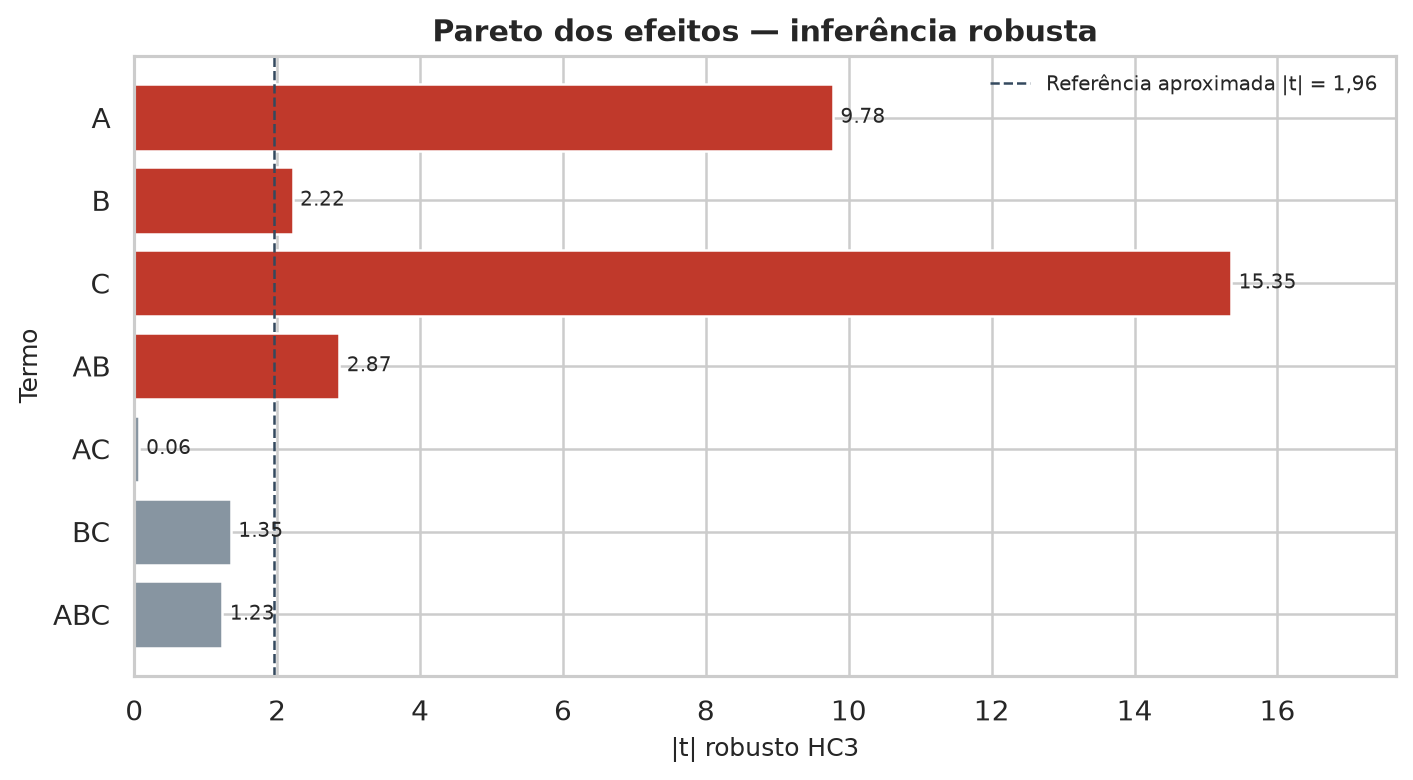
\includegraphics[width=\linewidth, height=0.68\textheight, keepaspectratio]{figuras/06_pareto_hc3.png}
            \vspace{-4pt}
            {\tiny \textbf{Figura 5:} Diagrama de Pareto com valores $|t|$ sob matriz sanduíche HC3.}
        \end{column}

        \begin{column}{0.44\textwidth}
            \begin{block}{Leitura do Diagrama}
                \begin{itemize}\setlength{\itemsep}{5pt}\small
                    %\item \textbf{Linha Crítica:} A reta tracejada em $|t| = 1.96$ delimita a significância bicaudal a 5\% ($\alpha = 0.05$).
                    \item \textbf{Linha Limiar ($\alpha = 0.05$):} A reta tracejada em $\vert{}t\vert{} = 1.96$ delimita a fronteira de significância estatística bicaudal.
                    %\item \textbf{Barras em Vermelho:} Termos que superam o limiar estatístico:
                    \item \textbf{Barras Destacadas (Significativas):} Termos que ultrapassam o limiar crítico:
                    \begin{itemize}\footnotesize
                        %\item $C$ ($|t| = 16.98$): relevância massiva;
                        %\item $A$ ($|t| = 10.49$): impacto pronunciado;
                        %\item $AB$ ($|t| = 2.87$): sinergia comprovada;
                        %\item $B$ ($|t| = 2.22$): efeito direto moderado.
                        \item $C$ ($\vert{}t\vert{} = 16.98$): fator dominante de maior impacto no desempenho.
                        \item $A$ ($\vert{}t\vert{} = 10.49$): forte penalidade associada ao uso passivo.
                        \item $AB$ ($\vert{}t\vert{} = 2.87$): interação significativa (amplificação do prejuízo).
                        \item $B$ ($\vert{}t\vert{} = 2.22$): impacto direto reduzido, mas estatisticamente relevante.
                    \end{itemize}
                    \item \textbf{Barras em Cinza:} Termos nulos ($BC, ABC, AC$) com $|t| < 1.96$.              


                    % O diagrama de Pareto confirma a hierarquia do experimento: o tempo de estudo dedicado ($C$) e o modo de uso da IA ($A$) conduzem o resultado acadêmico, enquanto interações secundárias não alteram o modelo.
                    
                \end{itemize}
            \end{block}
        \end{column}
    \end{columns}
\end{frame}

% ------------------------------------------------------------------------------
% Slide 19: Sensibilidade aos Cortes — Efeitos
% ------------------------------------------------------------------------------
\begin{frame}{18. Sensibilidade dos Efeitos a Regras de Corte Alternativas}
    \begin{columns}[c]
        \begin{column}{0.55\textwidth}
            \centering
            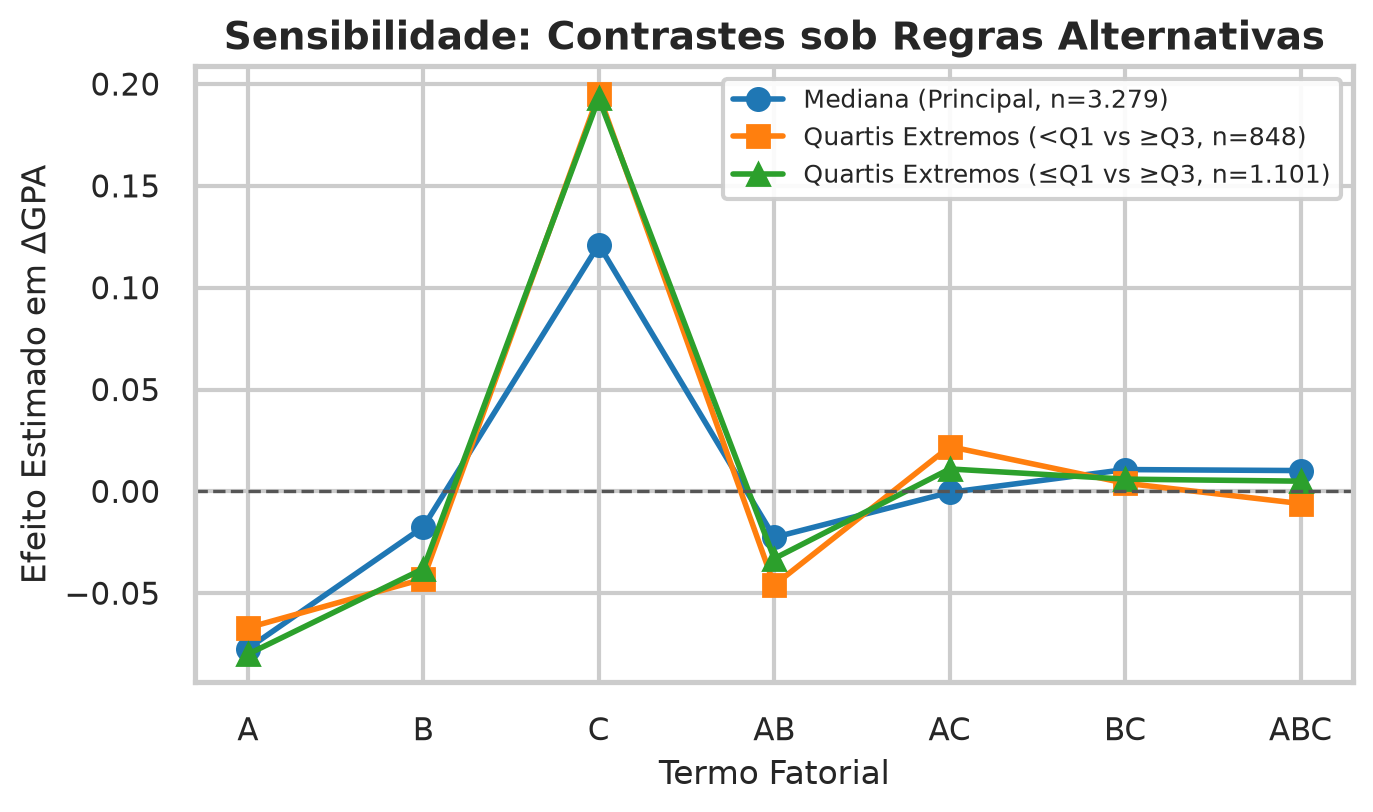
\includegraphics[width=\linewidth, height=0.68\textheight, keepaspectratio]{figuras/07_sensibilidade_efeitos.png}
            \vspace{-4pt}
            {\tiny \textbf{Figura 6A:} Estabilidade dos contrastes fatoriais sob diferentes regras de corte.}
        \end{column}

        \begin{column}{0.44\textwidth}
            \begin{block}{Medidas de Estabilidade}
                \begin{itemize}\setlength{\itemsep}{5pt}\small
                    %\item \textbf{Concordância de Sinais:} As três regras (Mediana, $<Q_1$ vs $\ge Q_3$ e $\le Q_1$ vs $\ge Q_3$) mantêm rigorosamente os mesmos sinais e hierarquias.
                    \item \textbf{Concordância de Sinais e Hierarquia:} As três regras (Mediana, Quartis $< Q_1$ vs. $\ge Q_3$ e $\le Q_1$ vs. $\ge Q_3$) mantêm rigorosamente a mesma direção e ordem de importância dos efeitos.
                    %\item \textbf{Efeito C Intensificado:} No corte por quartis extremos, o contraste de estudo salta de $+0.12$ para $\mathbf{+0.195}$, confirmando correlação positiva contínua.
                    \item \textbf{Efeito C Potencializado:} Nos extremos (quartis), o ganho por estudo tradicional salta de $\mathbf{+0.12}$ para $\mathbf{+0.195}$ pontos no GPA, confirmando a forte relação dos dados.  
                    %\item \textbf{Interação $A \times B$ Robusta:} Mantém-se negativa e significativa em todos os cenários.
                    \item \textbf{Interação $A \times B$ Robusta:} Permanece negativa e relevante em todos os cenários, comprovando a consistência da penalidade do uso passivo.  

                    %As descobertas do experimento são estáveis e robustas: a alteração dos critérios de divisão das variáveis não altera o comportamento dos fatores nem validações do modelo.
                    
                \end{itemize}
            \end{block}
        \end{column}
    \end{columns}
\end{frame}

% ------------------------------------------------------------------------------
% Slide 20: Sensibilidade — Tamanho Amostral
% ------------------------------------------------------------------------------
\begin{frame}{19. Sensibilidade: Amostra Efetiva por Regra de Dicotomização}
    \begin{columns}[c]
        \begin{column}{0.50\textwidth}
            \centering
            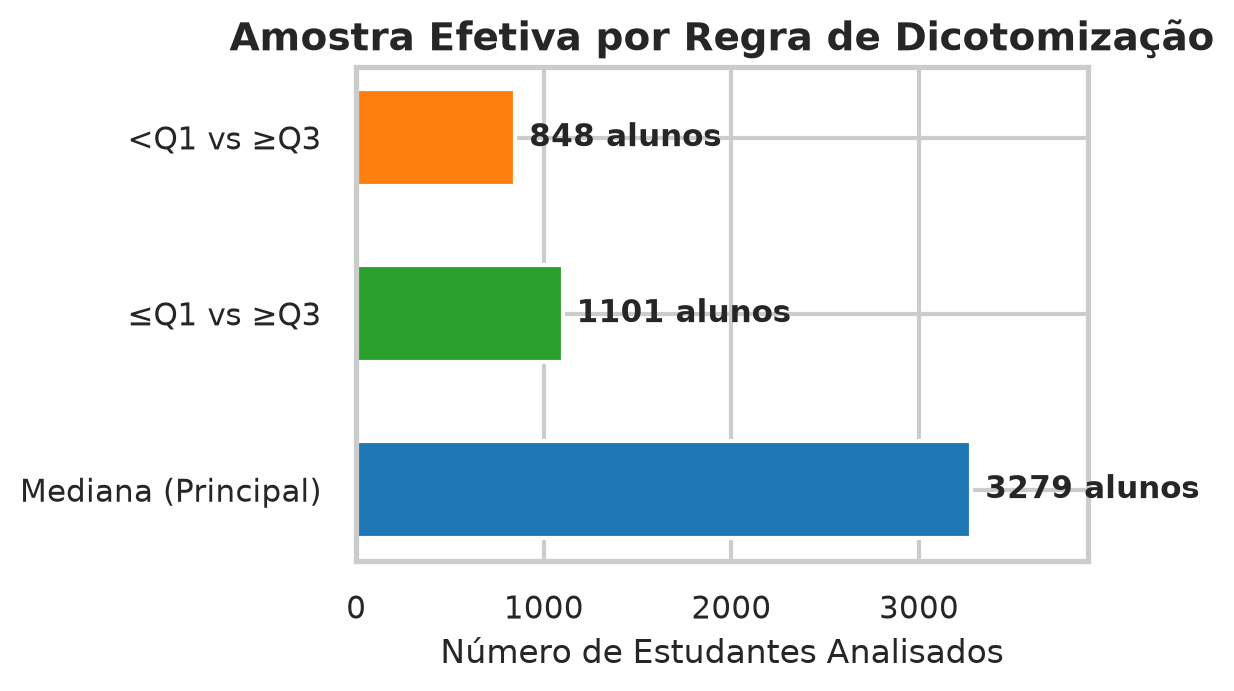
\includegraphics[width=\linewidth, height=0.68\textheight, keepaspectratio]{figuras/07_sensibilidade_amostra.png}
            \vspace{-4pt}
            {\tiny \textbf{Figura 6B:} Volume amostral disponível em cada regra de inclusão.}
        \end{column}

        \begin{column}{0.48\textwidth}
            \begin{block}{Medidas de Volume Amostral}
                \begin{itemize}\setlength{\itemsep}{5pt}\small
                    \item \textbf{Corte por Mediana ($Q_2$):} Utiliza $100\%$ da coorte elegível ($n = 3.279$ estudantes).
                    \item \textbf{Cortes Extremos por Quartis:} Descartam a faixa intermediária (50\% a 74\% da amostra), reduzindo $n$ para $848$ ou $1.101$.
                    \item \textbf{Poder Estatístico:} A regra da mediana foi mantida para evitar perda desnecessária de graus de liberdade.                    
                \end{itemize}
            \end{block}
        \end{column}
    \end{columns}
\end{frame}

% ------------------------------------------------------------------------------
% Slide 21: Avaliação Conclusiva da Hipótese Geral
% ------------------------------------------------------------------------------
\begin{frame}{20. Avaliação Preliminar da Hipótese Geral do Estudo}
    \begin{block}{Confronto Direto: Hipótese Geral vs. Evidências Empíricas}
        \centering
        \resizebox{\textwidth}{!}{%
        \renewcommand{\arraystretch}{1.15}
        \begin{tabular}{l c l}
            \toprule
            \textbf{Postulado na Hipótese Geral} & \textbf{Resultado} & \textbf{Evidência Experimental} \\
            \midrule
            Maior estudo tradicional eleva $\Delta$GPA & \cmark\ \textbf{Corroborado} & Efeito $C = +0.1211$ ($p < 0.0001$, dominante) \\
            Uso ativo supera o uso passivo de IA & \cmark\ \textbf{Corroborado} & Efeito $A = -0.0772$ ($p < 0.0001$, penalidade) \\
            Alta ansiedade reduz o $\Delta$GPA & \cmark\ \textbf{Corroborado} & Efeito $B = -0.0175$ ($p = 0.0268$, reduzido) \\
            Interação adversa entre passivo e ansiedade & \cmark\ \textbf{Corroborado} & Efeito $AB = -0.0226$ ($p = 0.0041$, sinergia) \\
            \midrule
            Interações com estudo tradicional ($AC, BC$) & \textbf{Não detectado} & Retas estritamente paralelas ($p > 0.17$) \\
            \bottomrule
        \end{tabular}%
        }
    \end{block}

    \vspace{2pt}

    \begin{block}{Síntese Preliminar}
        A hipótese geral foi \textbf{plenamente corroborada} em suas proposições ativas. A independência de $C$ em relação a $A$ e $B$ traz uma contribuição: o estudo tradicional protege os estudantes independentemente do seu perfil emocional ou tecnológico.
    \end{block}
\end{frame}

% ------------------------------------------------------------------------------
% Slide 22: Aprimoramentos para a Versão Final e Encerramento
% ------------------------------------------------------------------------------
\begin{frame}{21. Aprimoramentos para a Versão Final e Encerramento}
    \begin{columns}[T]
        \begin{column}{0.48\textwidth}
            \begin{block}{Ajustes Analíticos Planejados}
                \begin{itemize}\setlength{\itemsep}{5pt}\small
                    \item \textbf{Modelagem Contínua / ANCOVA:}
                    \begin{itemize}\footnotesize
                        \item Incluir as horas contínuas de estudo e ansiedade sem dicotomização.
                        \item Controlar explicitamente pelo $\text{GPA}_{\text{pré}}$ exato para medir ganhos marginais.
                    \end{itemize}
                    \item \textbf{Subpopulações STEM:}
                    \begin{itemize}\footnotesize
                        \item Investigar estabilidade entre subáreas (Engenharias vs Ciência da Computação).
                    \end{itemize}
                \end{itemize}
            \end{block}

            %\begin{block}{Recomendações Práticas}
            %    \begin{itemize}\footnotesize
            %        \item Desenvolver oficinas instrucionais para conscientizar discentes sobre uso ativo (depuração) e desestimular a cópia passiva.
            %    \end{itemize}
            %\end{block}
        \end{column}

        \begin{column}{0.48\textwidth}
            \begin{exampleblock}{Etapa Final }%(Peso: 50\%)}
                \begin{itemize}\setlength{\itemsep}{5pt}\small
                    \item Elaboração do \textbf{Relatório Final}% em LaTeX} no template oficial da disciplina.
                    \item Incorporação dos feedbacks recebidos nesta apresentação preliminar.
                    \item Redação do artigo científico completo (Introdução, Fundamentação, Métodos, Resultados Experimentais, Discussão e Conclusão).
                \end{itemize}
            \end{exampleblock}

            %\vspace{6pt}
            %\begin{center}
            %    \textbf{\large Muito Obrigado!} \\
            %    \medskip
                %{\small Dúvidas e Considerações da Banca} \\
                %\medskip
                %\textit{PPGCC --- UFOP}
            %\end{center}
        \end{column}
    \end{columns}
\end{frame}

\end{document}
